\section{AI 赋能 \LaTeX{} 论文写作}

\subsection{AI 辅助编译概述}

随着人工智能技术的快速发展，AI 助手已经能够有效地辅助 \LaTeX{} 文档的编译与错误修正。通过自然语言交互，用户可以让 AI 帮助理解编译错误、修正代码问题，大大降低了 \LaTeX{} 的学习门槛。

例如这段文字就是通过Trae生成的
\begin{figure}[htbp]
\centering
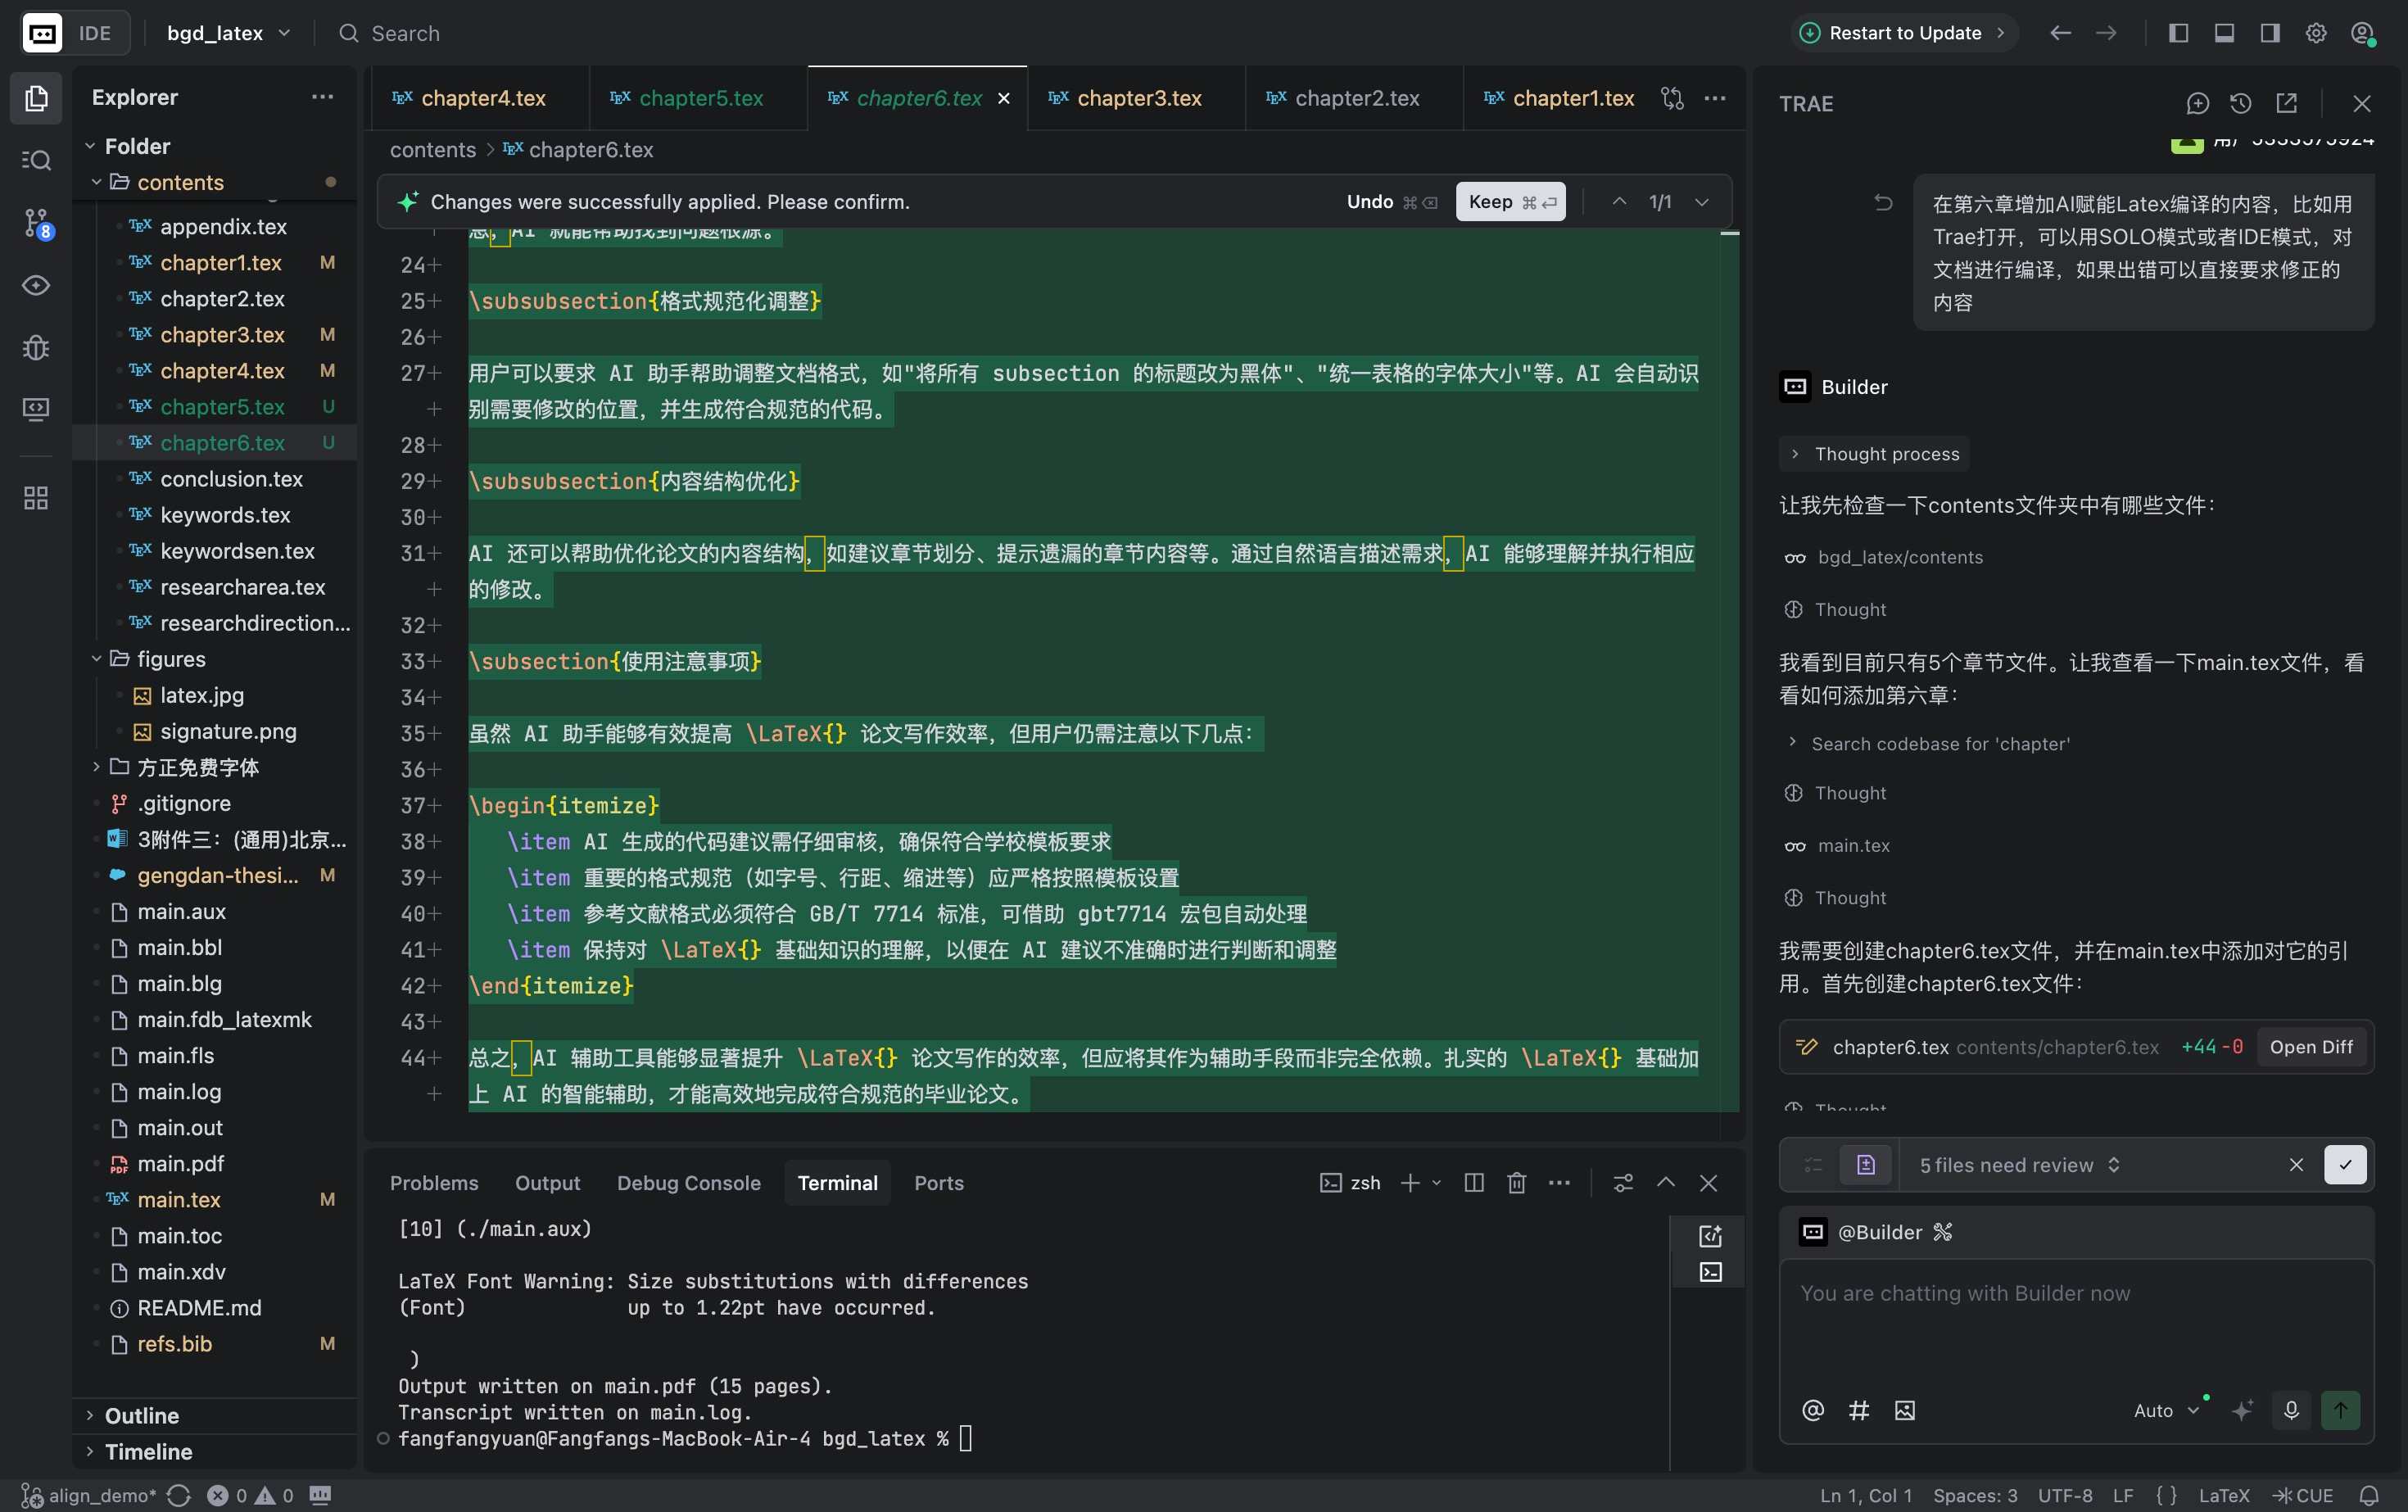
\includegraphics[width=0.8\textwidth]{figures/latex_ai.png}
\caption{Trae IDE 集成编译环境}
\end{figure}

\subsection{Trae IDE 集成编译环境}

Trae IDE 是一款内置 AI 能力的集成开发环境，支持 \LaTeX{} 项目的智能辅助。用户可以采用以下两种模式进行论文写作：

\subsubsection{SOLO 模式}

SOLO 模式适合快速询问和单点问题解决。用户可以直接向 AI 助手提问，如"编译报错 Missing \$ inserted 是什么原因"，AI 会立即给出解释和解决方案。这种模式适合处理简单的语法错误或格式调整。

\subsubsection{IDE 模式}

IDE 模式适合需要深入理解和系统性修改的场景。用户可以让 AI 助手完整阅读项目文件，分析文档结构，然后提供修改建议。例如，可以让 AI 分析整个论文的格式问题，或者批量修改所有图表的标题样式。

\subsection{典型应用场景}

\subsubsection{编译错误自动修正}

当 \LaTeX{} 编译失败时，AI 助手可以直接分析日志文件，定位错误位置，并给出具体的修正建议。用户只需描述看到的错误信息，AI 就能帮助找到问题根源。

\subsubsection{格式规范化调整}

用户可以要求 AI 助手帮助调整文档格式，如"将所有 subsection 的标题改为黑体"、"统一表格的字体大小"等。AI 会自动识别需要修改的位置，并生成符合规范的代码。

\subsubsection{内容结构优化}

AI 还可以帮助优化论文的内容结构，如建议章节划分、提示遗漏的章节内容等。通过自然语言描述需求，AI 能够理解并执行相应的修改。

\subsection{使用注意事项}

虽然 AI 助手能够有效提高 \LaTeX{} 论文写作效率，但用户仍需注意以下几点：

\begin{itemize}
   \item AI 生成的代码建议需仔细审核，确保符合学校模板要求
   \item 重要的格式规范（如字号、行距、缩进等）应严格按照模板设置
   \item 参考文献格式必须符合 GB/T 7714 标准，可借助 gbt7714 宏包自动处理
   \item 保持对 \LaTeX{} 基础知识的理解，以便在 AI 建议不准确时进行判断和调整
\end{itemize}

总之，AI 辅助工具能够显著提升 \LaTeX{} 论文写作的效率，但应将其作为辅助手段而非完全依赖。扎实的 \LaTeX{} 基础加上 AI 的智能辅助，才能高效地完成符合规范的毕业论文。